\documentclass[UTF8]{ctexart}
\usepackage{CJK}
\usepackage{amsmath}
\usepackage{geometry}
\usepackage{graphicx}
\usepackage{subfigure}
\usepackage{float}
\usepackage{algpseudocode}
\usepackage{algorithm}
\usepackage{algorithmicx}
\usepackage{caption,subcaption}
\usepackage{color}
\usepackage{mathtools}
\CTEXsetup[format={\Large\bfseries}]{section}
\title{Algorithm Design and Analysis: Assignment 4}
\author{钟赟 202028013229148}
\usepackage{geometry}
\geometry{left=2.5cm,right=2.5cm,top=2.5cm,bottom=2.5cm}

\newcommand{\fix}{\marginpar{FIX}}
\newcommand{\new}{\marginpar{NEW}}

\begin{document}
\maketitle
        
\section*{1 Traveling Trump Problem}
Suppose you are the U.S. presidential candidate Donald Trump, who want to hold election rallies in four swing states: Georgia(1), Pennsylvania(2), Michigan(3) and Florida(4). It is the
last day before election and because of shortage of funds, you need to save money and try to travel through the shortest path, visit each state exactly once and return to the starting
point. Distance between every two states can be writen as $c_{i j}, i \in[0,3], j \in[i, 4], i, j$ is integer.
Washington DC(0) is your starting point. Please formulate this problem as an ILP. (Hint: You can think about this problem in terms of the constraint that visiting each state exactly once. )
\section*{Solution}
设 $x_{ij}, i \in[0,3], j \in[i, 4]$ 表示每条边是否出现在最短路径上,$x_{ij} = 0, 1$ 。

LP formulation:

\begin{array}{rrrrrrrr}
	\min & \sum_{i \in[0,3], j \in[i, 4]} x_{i j} c_{i j} & \\
	\text {s.t.} & \sum_{i\in[0,3]} x_{i j} &\leq 2& \quad\text{for each}\quad j \in[i, 4]\\
	&  \sum_{j \in[i, 4]} x_{i j} &\leq 2& \quad\text{for each}\quad i \in[0,3]\\
	&  \sum_{j \in [0, 4]} x_{0 j} &= 2& \\
	& x_{i j} &= 0, 1 &\quad\text{for each}\quad i \in[0,3], j \in[i, 4]
\end{array}

\section*{2 Profit Maximization}
Your factory produces three kinds of product: A, B and C. All of them need two kinds of raw materials: nickel and aluminum. The profit and cost of each kind of product are shown in the following table.\\

\begin{tabular}{cccc}
	\hline Product & Profit(\$) & Nickel(kg) & Aluminum(kg) \\
	\hline A & 10 & 3 & 4 \\
	B & 5 & 3 & 2 \\
	C & 15 & 1 & 8 \\
	\hline
\end{tabular}
\\
You only have 100 kg of nickle and 200 kg of aluminum in stock. How to arrange production to maximize profits? Please formulate this problem as a LP and transform it into dual form.
Then you may solve both primal and dual problems using GLPK or Gurobi or other similar tools.

\section*{Solution}
设生产 $x_1$ 个 A 产品, $x_2$ 个 B 产品, $x_3$ 个 C 产品。

LP formulation(primal form):

\begin{array}{rrrrrrrr}
	\max & 10 x_{1} & + & 5 x_{2} & + & 15 x_{3}  & \\
	\text {s.t.} & 3 x_{1} & + & 3 x_{2} & + &  x_{3} & \leq & 100 \\
	& 4 x_{1} & + & 2 x_{2} & + & 8 x_{3} & \leq & 200 \\
	& x_{1} & , & x_{2} & , & x_{3} & \geq & 0
\end{array}

对偶问题:假设有另一个工厂有足够多的镍和铝材料,他们按照使用原材料的数量来支付钱款,求这家工厂最少花多少钱。设 $y_1, y_2$ 分别是本公司镍和铝每千克的报价。

Dual formulation:

\begin{array}{rrrrrrrr}
	\min & 100 y_{1} & + & 200 y_{2} & \\
	\text {s.t.} & 3 y_{1} & + & 4 y_{2} & \geq & 10 \\
	& 3 y_{1} & + & 2 y_{2} &\geq & 5 \\
	&  y_{1} & + & 8 y_{2} &\geq & 15 \\
	& y_{1} & ,&  y_{2}   & \geq & 0
\end{array}

使用 python 的 scipy 库函数来解线性规划问题,代码如下:

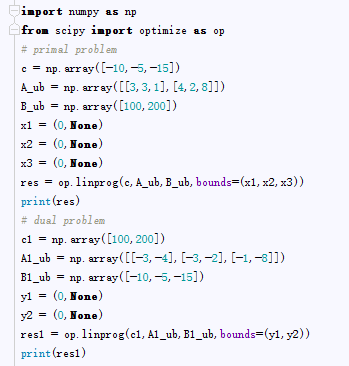
\includegraphics[width=0.6\textwidth]{code.png}

计算结果如图 (a) 和 (b)。

\begin{figure}
	\centering
	\subfigure[原问题的解]{
		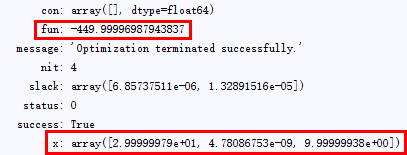
\includegraphics[width=0.5\textwidth]{res1.png}
	}
	\hspace{0.5in}
	\subfigure[对偶问题的解]{
		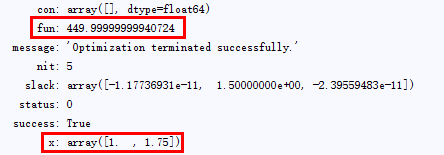
\includegraphics[width=0.5\textwidth]{res2.png}
	}
\end{figure}

由于原问题的约束条件是求解 max 问题,因此参数使用负数,得出的结果也为负数。由于 $x_1, x_2, x_3$ 和 $y_1, y_2$ 取值均为整数,故原问题的最优解为:
$x_1 = 30, x_2 = 0, x_3 = 10$ ,最大利润为 \$ 450 ;对偶问题的最优解为 $y_1 = 1, y_2 = 2,$ 最少花费为 \$ 450 。
\section*{3  Cutting Paper Minimization}
Your factory has expanded its bussiness. Suppose you have an unlimited number of large rolls of paper, of width $W$ meters per roll $(W$ is a positive integer). However, different $m$ customers demands are for smaller width of paper; in particular, customer $i$ needs $b_{i}$ rolls of paper of width $w_{i}, i=1,2, \ldots, m .$ We assume that $w_{i} \leq W$ for each $i,$ and each $w_{i}$ is an integer. Smaller rolls are obtained by slicing a large roll in a certain way. You can slice one roll of paper for different customers only if their total width does not exceed $W$.

The goal of you is to minimize the number of large rolls used while satisfying customer demand. Please formulate this problem as an ILP. Assume that there is no cost for slicing.
\section*{Solution}
设一卷长度为 $W$ 的纸共有 K 种分割方式,$x_{ij}$ 表示在第 $j$ 中分割方式下包含第 $i$ 个顾客需要的纸的数量,$y_j$ 表示每种分割方案执行的次数, $1\leq i \leq m, 1\leq j \leq K$。

LP formulation:

\begin{array}{rrrrrrrr}
	\min & \sum_{j = 1}^{K} y_j & \\
	\text {s.t.} & \sum_{j = 1}^{K} x_{ij} y_j & \geq & b_i & \text{for each} \quad i\in [1,m]\\
	& \sum_{i = 1}^{m} x_{ij}w_i &\leq & W & \text{for each} \quad j \in [1,K]\\
	& x_{ij} & \geq & 0 & \text{for each} \quad i\in [1,m], j\in [1,K]
\end{array}

\section*{4 Reformulation Problems with Absolute Values} 
Consider the problem:

\begin{array}{cl}
	\operatorname{minimize} & 2\left|x_{1}\right|+x_{2} \\
	\text { subject to } & x_{1}+x_{2} \geq 4
\end{array}

Please reformulate this problem as a LP without absolute values.

\section*{Solution}
绝对值 $\left|x_{1}\right|$ 可分解成正数部分 $x_{1}^+$ 和负数部分 $x_{1}^-$ ,即 $\left|x_{1}\right| = x_{1}^+ + x_{1}^-$ ,则 $x_{1} = x_{1}^+ - x_{1}^-$ , $x_{1}^+, x_{1}^- \geq 0$。

将上式代入,原问题可以转化成如下 LP 问题:

\begin{array}{rrrrrrrr}
	\min & 2 x_{1}^+ + 2 x_{1}^- +x_{2} \\
	\text { s.t. } & x_{1}^+ - x_{1}^- +x_{2} \geq& 4\\
	& x_{1}^+ , x_{1}^- \geq& 0
\end{array}

\section*{5 Lawyer Recruitment for Trump}
The U.S. presidential election is over, but Donald Trump refuses to accept defeat. Suppose you are Trump's election campaign manager and you are asked to recruit a group of lawyers for him to initiate litigation against the results. It is estimated that litigation will be initiated in $N$ states, and the $i(t h)$ state needs at least $L_{i}$ lawyers. The number of law firms is $F$. Lawyers from the $j(t h)$ law firm can offer legal services in several states $S_{j}$ and the recruitment fee for one lawyer from the $j(t h)$ law firm is $C_{j}$. Note that $S_{j}$ is a subset of $N=\{1,2, \cdots, n\}$ and the union of $S_{j}$ equals to $N$.

Your boss wants you to save money so your need to formulate this problem as an ILP and your goal is minimizing the recruitment fee of enough lawyers.
\section*{Solution}
设 $x_j^i$ 表示第 j 个法律公司派去第 i 个州的律师数量,  $x_j^i \geq 0, j \in [1, F], i \in N$。
$\sum_{i\in N}x_j^i$ 表示第 j 个公司派遣的律师总数, $\sum_{j=1}^{F}x_j^i$ 表示到达第 i 个州的律师总数。

ILP 问题形式:

\begin{array}{rrrrrrrr}
	\min & \sum_{j=1}^{F} ((\sum_{i\in N}x_j^i)& C_j) & \\
	\text {s.t.} & \bigcup\limits_{i\in N}& x_j^i &\subseteq& S_j & \text{for each}\quad j \in [1, F]\\
	& \sum_{j=1}^{F}&x_j^i &\geq& L_i& \text{for each}\quad i \in N \\
	& & x_j^i &\geq& 0 & \text{for each}\quad i \in N, j \in [1, F]
\end{array}

\end{document}


